\documentclass[11pt, a4paper]{article}

\usepackage{tikz}
\usepackage{float}
\usepackage{multicol}
\usepackage{graphicx}
\usepackage{amsfonts}
\usepackage[utf8]{inputenc}
\usepackage[english]{babel}
\usepackage[margin=2cm]{geometry}

\setlength{\columnsep}{5mm}
\graphicspath{{graphs/}}

\title{Exoplanets detection using auto-tuned random forest}
\author{Lorenzo Loconte}

\begin{document}

\maketitle
\begin{abstract}
  This work consists of identifying exoplanets using random forest which hyperparameters are optimized.
  The model is trained using the processed data that come from the NASA's Kepler project of discovering exoplanets (e.g. planets outside our solar system).
  The hyperparameters of the model are optimized and cross-validated with random search, a simple yet effective scalable method for hyperparameters optimization.
  The data used in this work can be found at \textbf{https://exoplanetarchive.ipac.caltech.edu}.
\end{abstract}
\vspace{5mm}

\begin{multicols}{2}
\section{Introduction}
  \paragraph{Kepler Object of Interest}
    The dataset used to train the model is composed by a list of features regarding exoplanets. Each tuple have a label indicating if the corresponding exoplanet is candidate, false positive or confirmed. The selected features for the classification task are the following:
    \begin{enumerate}
      \item Orbital Period [days]
      \item Impact Parameter
      \item Transit Duration [hrs]
      \item Transit Depth [ppm]
      \item Planet-Star Radius Ratio
      \item Fitted Stellar Density [g/cm**3]
      \item Planetary Radius [Earth radii]
      \item Orbit Semi-Major Axis [AU]
      \item Inclination [deg]
      \item Equilibrium Temperature [K]
      \item Insolation Flux [Earth flux]
      \item Stellar Effective Temperature [K]
      \item Stellar Surface Gravity [log10(cm/s**2)]
      \item Stellar Radius [Solar radii]
      \item Stellar Mass [Solar mass]
      \item RA [decimal degrees]
      \item Dec [decimal degrees]
      \item Kepler-band [mag]
    \end{enumerate}
    The tuples corresponding to features of candidate exoplanets are discarded. Only confirmed and false positive ones are included in the train and the test sets in order to reduce noises and improve the learning process. The preprocess method applied to the dataset is the standard normalization.
  \paragraph{Random Forests and Hyperparameters}
    The model used for the classification task is a random forest, an ensemble of random decision trees. The prediction of the random forest is computed as the mode of each tree's classification. Each tree of the forest is trained on a subset of the features and samples.
    The hyperparameters of the random forest are optimized and cross-validated using random search. The following hyperparameters are optimized:
    \begin{itemize}
      \item Number of estimators (e.g. the number of trees)
      \item The minimum number of samples required to split an internal node
      \item The percentage of features to use for each tree
    \end{itemize}

\section{Hyperparameters Tuning}
  The hyperparameters optimization task consists to find the hyperparameters for a model that maximize a certain score. In this work we refer to hyperparameters as the ones that cannot be trained (e.g. the ones described in the previous section).
  There are a lot of different techniques for hyperaparameters optimization, some of them are the following:
  \begin{itemize}
    \item Random Search
    \item Grid Search
    \item Hyperbands
    \item Genetic methods
    \item Bayesian optimization
  \end{itemize}
  In this work, given the restricted hyperparameters search space, we used random search as the hyperparameters algorithm. It's a simple method that consists of random sampling some points in the hyperparameters space and cross-validating them on the validation set. After some iterations we pick the best hyperparameters point corresponding to the best model.
  Even if it is a simple algorithm, it is well scalable on multiple CPUs because every point in the hyperparameters space is independent from the others.
  In this work the hyperparameters search space can be defined formally as:
  \[\Omega=\mathbb{N}^{*}\times\mathbb{N}^{*}\times(0,1]\]
  Table \ref{table:hyperparameters} shows the subset of the search space used in this work.
  
  \begin{table}[H]
    \centering
    \begin{tabular}{|c c|}
      \hline
      Hyperparameters & Values \\
      \hline\hline
      Estimators number & $\{10,20,...,120\}$ \\
      \hline
      Minimum samples to split & $\{2,4,8,16,32\}$ \\
      \hline
      Features percentage & $\{0.1,0.2,...,1.0\}$ \\
      \hline
    \end{tabular}
    \caption{Hyperparameters space subset}
    \label{table:hyperparameters}
  \end{table}

  The optimization task consists to find a point in the hyperparameters space:
  \[\omega=(n, k, p)\in\Omega\]
  where $n$ is the number of estimators, $k$ is the minimum samples to split, $p$ is the features percentage for each tree, such that the random forest built from these hyperparameters maximize a certain score. The choice of this score is dependent from the task. For simplicity we use the $F_{1}$ score (e.g. we want to maximize both \textit{Precision} and \textit{Recall}).

\section{Conclusion and Results}
  As you can see from Table \ref{table:confusion} the false positives count (the number of examples, which are predicted as exoplanets, that are not) and the false negatives count (the number of actual exoplanets not being discovered), are pretty low.
  \begin{table}[H]
    \centering
    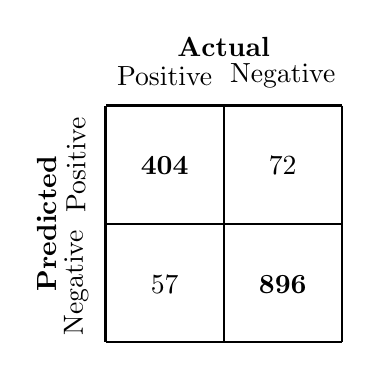
\begin{tikzpicture}[scale=1.5]
      % Draw the box
      \draw[thick] (0, 0) -- (2, 0);
      \draw[thick] (0, 0) -- (0, 2);
      \draw[thick] (2, 2) -- (2, 0);
      \draw[thick] (2, 2) -- (0, 2);
      \draw[thick] (0, 1) -- (2, 1);
      \draw[thick] (1, 0) -- (1, 2);
      % Draw the headers
      \node[rotate=0] (h1) at (1, 2.5) {\textbf{Actual}};
        \node[rotate=0] (h11) at (0.5, 2.25) {Positive};
        \node[rotate=0] (h12) at (1.5, 2.25) {Negative};
      \node[rotate=90] (h2) at (-0.5, 1) {\textbf{Predicted}};
        \node[rotate=90] (h21) at (-0.25, 1.5) {Positive};
        \node[rotate=90] (h22) at (-0.25, 0.5) {Negative};
      % Draw the category values
      \coordinate[label={\textbf{404}}] (PP) at (0.5, 1.33);
      \coordinate[label={ 57}] (NP) at (0.5, 0.33);
      \coordinate[label={ 72}] (PN) at (1.5, 1.33);
      \coordinate[label={\textbf{896}}] (NN) at (1.5, 0.33);
    \end{tikzpicture}
    \caption{Confusion matrix over the test set.}
    \label{table:confusion}
  \end{table}

  As you can see from Table \ref{table:benchmark} the auto-tuned random forest used in this work obtained a similar precision to other models but a way better recall. For this task we want to have a better recall because we want to maximize the number of actual exoplanets discovered.
  In the end we present Table \ref{table:importances} that shows the importances (and their standard deviations) of the first five out eighteen features used.
\end{multicols}

  \begin{table}
    \centering
    \begin{tabular}{|c c c c c|}
      \hline
      Model & Settings & Precision & Recall & $F_{1}$  \\
      \hline\hline
      k-NN & k=5, euclidean norm, uniform weights & 0.926 & 0.835 & 0.878 \\
      \hline
      SVC & regularizer=1.0, rbf kernel, gamma scale & 0.929 & 0.883 & 0.905 \\
      \hline
      2-layer NN & 100 hidden units, relu activation, adam & 0.938 & 0.921 & 0.928 \\
      \hline
      \textbf{Random Forest} & \textbf{auto-tuned hyperparameters} & \textbf{0.940} & \textbf{0.926} & \textbf{0.933} \\
      \hline
    \end{tabular}
    \caption{Precision, recall and $F_{1}$ metrics of several models for comparison. The hyperparameters of \textit{Random Forest} were optimized automatically. In this table it was built with the following hyperparameters: 100 estimators, 2 minimum samples to split and 5 features per tree.}
    \label{table:benchmark}
  \end{table}

  \begin{table}
    \centering
    \begin{tabular}{|c c c|}
    \hline
    Feature \# & Description & Importance \\
    \hline\hline
    7 & Planetary Radius & 0.15 \\
    5 & Planet-Star Radius Ratio & 0.11 \\
    1 & Orbital Period & 0.09 \\
    6 & Fitted Stellar Density & 0.07 \\
    8 & Orbit Semi-Major Axis & 0.07 \\
    \hline
    \end{tabular}
    \caption{Features importances in descending order.}
    \label{table:importances}
  \end{table}

\newpage
\begin{thebibliography}{9}
  \bibitem{example}
    Loconte Lorenzo
    \textit{This Work}, 2020.
\end{thebibliography}

\end{document}
